% !TeX TXS-program:compile = txs:///pdflatex/[--shell-escape]
\documentclass[10pt,landscape,a4paper]{article}
\usepackage[table]{xcolor}
\usepackage[normalem]{ulem}
\usepackage{tikz}
\usetikzlibrary{shapes,positioning,arrows,fit,calc,graphs,graphs.standard}
\usepackage[nosf]{kpfonts}
\usepackage[t1]{sourcesanspro}
\usepackage{multicol}
\usepackage{wrapfig}
\usepackage[top=1mm,bottom=1mm,left=1mm,right=1mm]{geometry}
\usepackage[framemethod=tikz]{mdframed}
\usepackage{microtype}
\usepackage{tabularx}
\usepackage{hhline}
\usepackage{makecell}
\usepackage{mathtools}
\usepackage{subfig}
\usepackage{listings}
\usepackage{soul}
\usepackage{amsmath,amsthm,amsfonts,amssymb}

\graphicspath{ {./img/} }

\DeclarePairedDelimiter{\ceil}{\lceil}{\rceil}

\definecolor{myblue}{cmyk}{1,.72,0,.38}

\pgfdeclarelayer{background}
\pgfsetlayers{background,main}

\renewcommand{\baselinestretch}{.8}
\pagestyle{empty}

\let\counterwithout\relax
\let\counterwithin\relax
\usepackage{chngcntr}
\usepackage{verbatim}
\usepackage{etoolbox}
\makeatletter
\preto{\@verbatim}{\topsep=0pt \partopsep=0pt }
\makeatother

\counterwithin*{equation}{section}
\counterwithin*{equation}{subsection}
\usepackage{enumitem}
\newlist{legal}{enumerate}{10}
\setlist[legal]{label*=\arabic*.,leftmargin=3mm}
\setlist[itemize]{leftmargin=4mm}
\setlist[enumerate]{leftmargin=4.5mm}
\setlist{nosep}
\usepackage{minted}

\newenvironment{descitemize} % a mixture of description and itemize
{\begin{description}[leftmargin=*,before=\let\makelabel\descitemlabel]}
    {\end{description}}
\newcommand{\descitemlabel}[1]{%
    \textbullet\ \textbf{#1}%
}
\makeatletter

\renewcommand{\section}{\@startsection{section}{1}{0mm}%
    {.2ex}%
    {.2ex}%x
    {\color{myblue}\sffamily\small\bfseries}}
\renewcommand{\subsection}{\@startsection{subsection}{1}{0mm}%
    {.2ex}%
    {.2ex}%x
    {\sffamily\bfseries}}
\renewcommand{\subsubsection}{\@startsection{subsubsection}{1}{0mm}%
    {.2ex}%
    {.2ex}%x
    {\rmfamily\bfseries}}

\makeatother
\setlength{\parindent}{0pt}
\setminted{tabsize=2, breaklines}
% Remove belowskip of minted
\setlength\partopsep{-\topsep}

\newcolumntype{a}{>{\hsize=1.5\hsize}X}
\newcolumntype{b}{>{\hsize=.25\hsize}X}

\setlength\columnsep{10pt}
\setlength\columnseprule{0pt}
\begin{document}
\abovedisplayskip=0pt
\abovedisplayshortskip=0pt
\belowdisplayskip=0pt
\belowdisplayshortskip=0pt
%\scriptsize
\tiny
\begin{multicols*}{4}
	\raggedcolumns
	\section{Dynamic Programming}
	\begin{itemize}
		\item Typically built on the \textbf{divide-and-conquer} paradigm where we divide the input instance into 2 or more parts (of equal sizes), solve the same problem for each smaller instance recursively and combine the solutions to get solution of original instance
		\item Fibonacci is commonly used to demonstrate DP as the recursive algorithm takes $2^{(n-2)/2} \approx \phi^n$ time to run if using unoptimized recursion and takes only $5n$ time to run using iterative algorithm
		\item DP uses memoization technique to prune away recursion tree to reduce the number of repeated calculation
	\end{itemize}
	\subsection{Main Concepts}
	\begin{itemize}
		\item \textbf{cut-and-paste proof} $\rightarrow$ proof by contradiction - suppose you have an optimal solution. Replacing ("cut") subproblem solutions with this subproblem solution ("paste" in) should improve the solution. If the solution doesn’t improve, then it’s
		      not optimal (contradiction)
		\item \textbf{optimal substructure} - optimal substructure to a problem (instance) contains optimal solutions to subproblems
		\item \textbf{Overlapping subproblems}: recursive solution contains a "small" number of distinct subproblems repeated many times
		\item \textbf{Tips}: look at the \textcolor{red}{prefix} of the problem!! DP usually generates solutions based on what is already calculated. It generally also involves some sort of decision you have to make (e.g. either you take or you don't take)
	\end{itemize}
	\subsection{Longest Common Subsequence}
	\begin{itemize}
		\item Definition of Subsequence: for a sequence $A : a_1,a_2,...,a_n$ stored in an array, $C$ is a subsequence of $A$ if we can obtain $C$ by removing 0 or more elements from $A$
		\item \textbf{Problem}: given two sequences $A[1..n]$ and $B[1..m]$,
		      compute the longest sequence $C$ such that $C$ is a subsequence of $A$ and $B$
	\end{itemize}
	\subsubsection{Brute Force Approach}
	\begin{itemize}
		\item Check all possible subsequence of $A$ to see if it is also a subsequence of $B$, then output longest one
		\item Runtime will be \textbf{$O(m2^n)$}, where $m$ is the time taken to check whether a subsequence of $A$ is a subsequence of $B$ and there are $2^n$ possible subsequence since each char in $A$ we can choose to either take or we don't
	\end{itemize}
	\subsubsection{Recursive Formulation}
	\begin{itemize}
		\item Let $LCS(i,j)$ be the LCS of $A[1..i]$ and $B[1..j]$
		\item \textbf{Base case}: $LCS(i,0)=\emptyset, \forall i$, $LCS(0, j)=\emptyset, \forall j$
		\item \textbf{General case} (optimal substructure):
		      \begin{itemize}
			      \item if $a_n=b_m$ $\rightarrow$ $LCS(n,m) = LCS(n-1, m-1) ::a_n$, where $::a_n$ mean that we concatenate $a_n$ to the subsequence in $LCS(n-1,m-1)$
			      \item \textbf{Cut-and-paste argument}: Suppose $S$ returned by $LCS(n-1,m-1)$ is optimal solution for $A[1..n-1], B[1..m-1]$, we could just append $a_n$ to $S$ to get a subsequence with a length increased by 1, thus $S$ could not have been the largest subsequence
			      \item if $a_n\neq b_m$ $\rightarrow$ $LCS(n,m)=max(LCS(n-1,m), LCS(n,m-1))$
		      \end{itemize}
		\item \textbf{Simplified Problem}:
		      \begin{itemize}
			      \item $L(n,m)$: Length of LCS of $A[1..n]$ and $B[1..m]$
			      \item $L(n,m)=0$ if $n$ or $m$ = 0
			      \item if $a_n=b_m$ $\rightarrow$ $L(n,m)=L(n-1,m-1) + 1$
			      \item if $a_n\neq b_m \rightarrow L(n,m)=max(L(n,m-1), L(n-1, m))$
		      \end{itemize}
		\item \textbf{Analysis}:
		      \begin{itemize}
			      \item $T(n,m)=T(n-1, m) + T(n, m-1) + \Theta(1)\rightarrow2^n$
			      \item However, there is effectively only $(n+1)\times (m+1)$ subproblems
			      \item Could be solved in $O(nm)$ using bottom up approach with extra space of $O(min(n,m))$ to store intermediate results
		      \end{itemize}
	\end{itemize}
	\subsection{Knapsack Problem}
	\begin{itemize}
		\item \textbf{Input}: $(w_1,v_1), (w_2,v_2),...,(w_n,v_n)$ and capacity $W$
		\item \textbf{Output}: subset $S\subseteq\{1,2,...,n\}$ that maximises $\sum_{i\in S}v_i, s.t. \sum_{i\in S}w_i\leq W$
		\item \textbf{Naive solution}: runs in $2^n$ time since there are $2^n$ possible combinations
	\end{itemize}
	\subsubsection{Recursive Solution}
	\begin{itemize}
		\item Let $m(i,j)$ be the maximum value that can be obtained using the first $\{1,2,...,i\}$ items with total weight $\leq j$
		\item $m(i,j)=\begin{cases}
				      0,                                  & \text{if } i=0 \text{ or } j=0 \\
				      max(m(i-1, j-w_i) + v_i, m(i-1,j)), & \text{if } w_i\leq j           \\
				      m(i-1,j),                           & \text{otherwise}
			      \end{cases}$
		\item \textbf{Analysis}: $O(nW)$, which is a pseudo-polynomial algorithm as $W$ can be represented in $O(\lg W)$ bits and $n$ can be represented in $O(\lg n)$ bits.
		\item Also a suboptimal solution as it depends on $W$
	\end{itemize}
	\subsection{Changing Coins}
	\begin{itemize}
		\item \textbf{Problem}: use the fewest number of coins to make up $n$ cents using denominations $d_1, d_2,...,d_n$. Let $M[j]$ be the fewest number of coins needed to change $j$ cents.
		\item \textbf{Optimal Substructure}: $M[j]=\begin{cases}
				      1+\underset{i\in [k]}{\min}M[j-d_i], & j > 0 \\
				      0,                                   & j=0   \\
				      \infty,                              & j < 0
			      \end{cases}$
		\item \textbf{Proof}: Suppose $M[j]=t$, meaning $j=d_{i_1}+d_{i_2}+...+d_{i_t}$ for some $i_1,...,i_t\in \{1,..,k\}$. Then if $j'=d_{i_1}+d_{i_2}+...+d_{i_{t-1}}$, $M[j']=t-1$ because otherwise if $M[j']<t-1$, by cut-and-paste argument, $M[j] < t$
		\item \textbf{Runtime}: $O(nk)$, for $n$ cents and $k$ denominations
	\end{itemize}
	\section{Greedy Algorithms}
	\begin{itemize}
		\item In DP, there are often choices to be made which leads to multiple subproblems (branching)
		\item In Greedy Algorithms, we\textbf{ only solve 1 subproblem} at each step which could result in greedy algorithms beating divide-and-conquer and DP \textbf{when it works}
		\item To solve Greedy Algorithm problems, look out for the \textbf{Optimal Substructure} (cut-and-paste argument) and \textbf{Greedy-Choice property} $\rightarrow$ locally optimal solution is globally optimal
	\end{itemize}
	\subsection{Fractional Knapsack}
	\begin{itemize}
		\item \textbf{Input}: $(w_1,v_1), (w_2,v_2),...,(w_n),v_n$ and capacity $W$
		\item \textbf{Output}: Weights $x_1,...,x_n$ that maximizes $\sum_{i}x_i\cdot \dfrac{x_i}{w_i}$, subject to $\sum_{i}x_i\leq W$ and $0\leq x_j\leq w_j, \forall j\in [n]$
	\end{itemize}
	\subsubsection{Optimal Substructure property}
	\begin{itemize}
		\item If we remove $w$ kgs of one item $j$ from the optimal knapsack, then the remaining load must be the optimal knapsack weighing at most $W-w$ kgs that one ca ntake from the $n-1$ original items and $w_j-w$ kgs of item $j$
		\item \textbf{Cut-and-paste proof}: Suppose some $(y_1,...,y_i,...,y_n)$ weighed $\leq (W-w)$ and had better value than $(x_i,...,x_i-w,...,x_n)$ (optimal solution), then $(y_1,...,y_i+w,...,y_n)$ weighs $\leq$ W and has better value than $(x_1,...,x_i,...,x_n)$ $\rightarrow$ Contradiction!
	\end{itemize}
	\subsubsection{Greedy-choice Property}
	\begin{itemize}
		\item Let $j^*$ be the item with the maximum value/kg, $v_j/w_j$. Then there exists an optimal solution that contains $min(w_{j^*}, W)$ kgs of item $j^*$
		\item \textbf{"Exchange argument"}: Suppose an optimal knapsack contains $(x_1+x_2+...+x_n) = min(w_{j^*}, W)$ of items $(1,...,n)$, we could replace this with $min(w_{j^*}, W)$ of item $j^*$ which does not change the weight but value will also not decrease since $j^*$ has max weight/value ratio $\rightarrow$ knapsack stays optimal
	\end{itemize}
	\subsubsection{Analysis}
	\begin{itemize}
		\item Algorithm will be to sort items in terms of their weight/value ratio and keep choosing the item with highest weight/value ratio until we reach the target weight
		\item Sorting takes $O(n\lg n)$ so greedy fractional knapsack takes $O(n\lg n)$
	\end{itemize}
	\subsection{Minimum Spanning Tree}
	\subsubsection{Graph Review}
	\begin{itemize}
		\item In any graph, $|E|=O(|V|^2)$
		\item Degree of vertex is the number of edges containing $v$
		\item \textbf{Handshaking Lemma}: In any graph, $\sum_{v\in V}\deg(v)=2\cdot|E|$ $\rightarrow$ total number of degree = 2 $\cdot$ number of edges
	\end{itemize}
	\subsubsection{Problem Definition}
	\begin{itemize}
		\item \textbf{Input}: Connected graph $G=(V,E)$ and weight function $w$ (weight is on edges)
		\item \textbf{Output}: spanning tree of $G$ with minimum weight
	\end{itemize}
	\subsubsection{Optimal Substructure}
	\begin{itemize}
		\item Let $T$ be a MST. Remove any edge $(u,v)\in T$, then $T$ is partitioned into 2 subsets $T_1$ and $T_2$ which are both MSTs
		\item \textbf{Cut-and-paste argument}: If $T_1'$ has a lower MST weight than $T_1$, then we could create a MST $T'=\{u,v\}\cup T_1'\cup T_2$ which has a lower weight than $T$ for $G$ $\rightarrow$ Contradiction!
	\end{itemize}
	\subsubsection{Greedy Choice Property}
	\begin{itemize}
		\item Let $T$ be the MST of $G=(V,E)$, and let $A\subseteq V$. Supposed that $(u,v)\in E$ is the least weight edge connecting $A$ to $V - A$, then $(u,v)\in T$
	\end{itemize}
	\subsection{Prim's Algorithm}
	\begin{itemize}
		\item Maintain $V-A$ as a priority queue $Q$. At each step, add the least-weight edge from the tree to some vertex outside the tree then relax
	\end{itemize}
	\begin{center}
		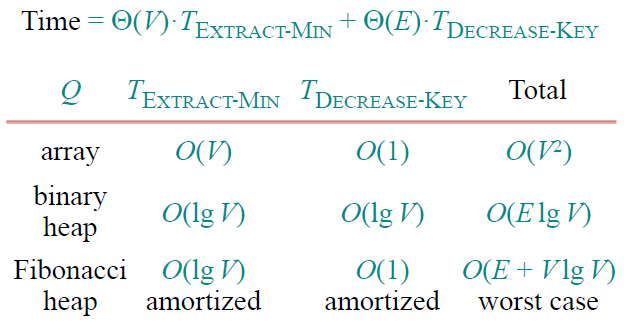
\includegraphics[width=0.4\columnwidth]{analysis_prims}
	\end{center}
	\subsection{Kruskals Algorithm}
	\begin{itemize}
		\item Basic idea is to add least-weight edge that does not cause cycle to form.
		\item Running time of $O(E\lg v)$, works better for sparse trees where $|E|\approx|V|$
	\end{itemize}
	\section{Incremental Algorithms}
	\subsection{Flow Networks}
	\begin{itemize}
		\item Directed graph $G=(V,E)$ in which each edge $(u,v)\in E$ has a capacity $c(u,v)\geq 0$, if $(u,v)\notin E, c(u,v)=0$
		\item Assumes no self-loops and not anti-parallel edges
		\item Flow is a function $f$ that assigns a number $f(u,v)$ to each edge - the flow from $u$ to $v$
		\item Constraints:
		      \begin{enumerate}
			      \item \textbf{Capacity}: each edge has a capacity constraint that states that flow cannot exceed capacity
			      \item \textbf{Flow conservation}: For every vertex - Flow into vertex must equal flow out of vertex
		      \end{enumerate}
		\item Value of flow, $|f|$ is the total flow from source to target
	\end{itemize}
	\subsection{Max Flow Problem}
	\begin{itemize}
		\item Given a flow network $G=(V,E)$ and capacities $c$, find a flow that maximizes $|f|$
		\item Solved using Ford-Fulkerson Algorithm (won't return non-integer values)
		      \begin{enumerate}
			      \item Start with $f(u,v)=0$ for all $(u,v)$
			      \item While there is a path $p$ from $s$ to $t$ in $G_f$:
			            \begin{enumerate}
				            \item Let $m=min_{(u,v)\in p}c_f(u,v)$
				            \item For each $(u,v)\in p$
				                  \begin{enumerate}
					                  \item If $(u,v)\in E$: increment  $f(u,v)$ by $m$ (increment if edge in $G$)
					                  \item If $(v,u\in E)$: decrement $f(v,u)$ by $m$ (decrement if edge not in $G$)
				                  \end{enumerate}
			            \end{enumerate}
		      \end{enumerate}
		\item \textbf{Runtime}: $O(|E|\cdot |f_{max}|)$ if we use depth-first search, where $f_{max}$ is the maximal flow.\\
		      $O(|V||E|^2)$ if we use BFS (Edmonds-Karp Algorithm), $O(|E||V|^2)$ if we use Dinic's
		\item To prove correctness, need to show:
		      \begin{itemize}
			      \item If $f$ is a valid flow (satisfies capacity constraint and flow conservation), it remains a valid flow after the changes made in step 2(b)
			      \item If there is no path $p$ from $s$ to $t$ in $G_f$, then $f$ is maximal flow
		      \end{itemize}
	\end{itemize}
	\begin{center}
		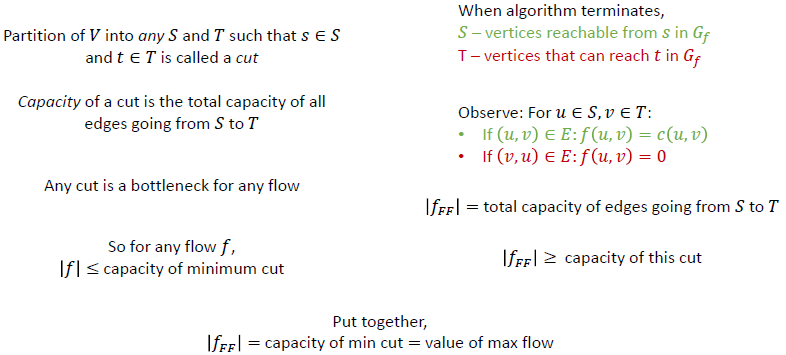
\includegraphics[width=0.6\columnwidth]{flows-and-cuts}
	\end{center}
	\subsubsection{Application: Bipartite Matching}
	\begin{itemize}
		%		\item \textbf{Matching}: A subset of edges such that each vertex is part of at most 1 edge
		\item Problem is the find the largest number of edges a matching can have
		\item Problem could be modeled by connecting the bipartite graph with a source node that points to each of the "left" nodes and a sink node that all "right" nodes point to
		\item Any \textbf{integer} flow corresponds to some matching
	\end{itemize}
	\section{Linear Programming}
	Linear programming is a mathematical modeling technique in which a \textbf{linear function (objective) is maximized or minimized} when subjected to various constraints. The optimal solution can be found in $poly(n,m)$ time and is quite efficient to solve in practice.
	\subsection{"Standard form" of LP}
	\begin{center}
		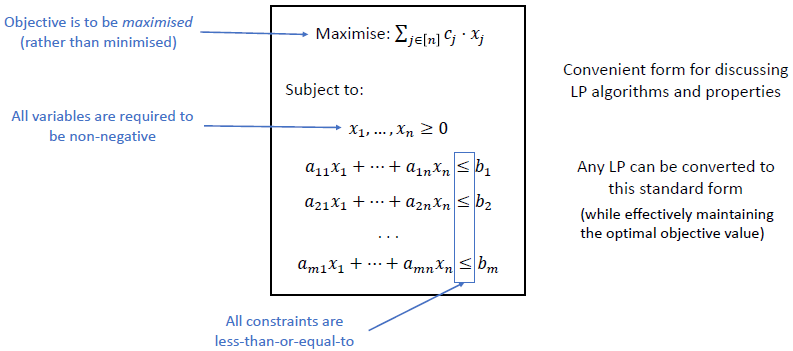
\includegraphics[width=0.7\columnwidth]{lp-sf}
	\end{center}
	\subsubsection{Converting to Standard Form}
	\begin{center}
		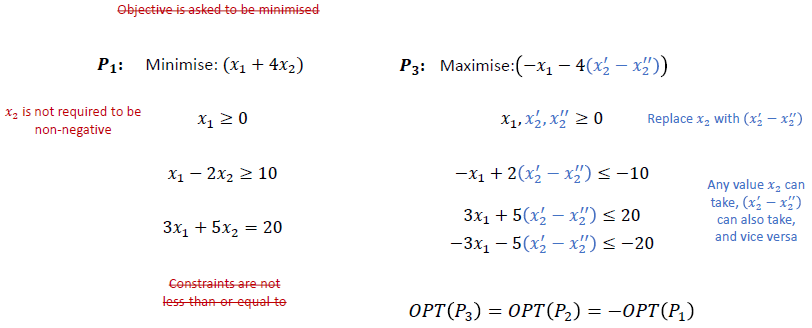
\includegraphics[width=0.7\columnwidth]{convert-lp}
	\end{center}
	\subsection{Example: Max Flow}
	\begin{itemize}
		\item Variables defined as $f(u,v)$ for every $(u,v)\in E$
		\item Maximize: $\sum_{v\in Neigh(s)}f(s,v)$
		\item Subjected to:
		      \begin{itemize}
			      \item $\forall(u,v)\in E: f(u,v)\geq 0$
			      \item $\forall(u,v)\in E: f(u,v)\leq c(u,v)$ (capacity constraint)
			      \item $\forall u\in V \backslash \{s,t\}: \sum_{v\in V}f(v,u)=\sum_{v\in V}f(u,v)$ (flow conservation)
		      \end{itemize}
		\item Can solve Max Flow problem using LP in $poly(|V|,|E|)$ which is not as fast as dedicated algorithms for Max Flow
	\end{itemize}
	\subsection{Example: Min-Cost Flow}
	\begin{center}
		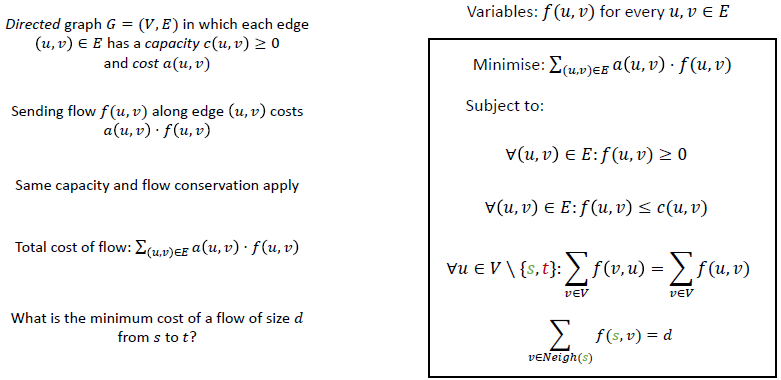
\includegraphics[width=0.7\columnwidth]{min-cost-flow}
	\end{center}
	\subsection{Example: Multicommodity Flow}
	\begin{center}
		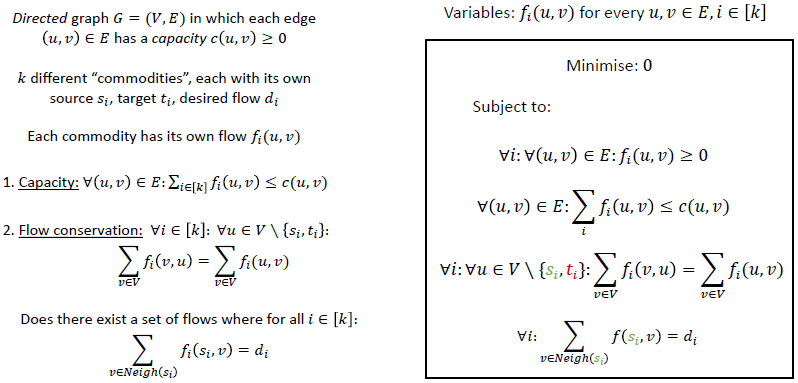
\includegraphics[width=0.7\columnwidth]{multicommodity-flow}
	\end{center}
	* Note that we are optimizing" a constant function here as this is a decision problem
	\subsection{Simplex Algorithm}
	Linear programs can be represented as a graph
	\begin{center}
		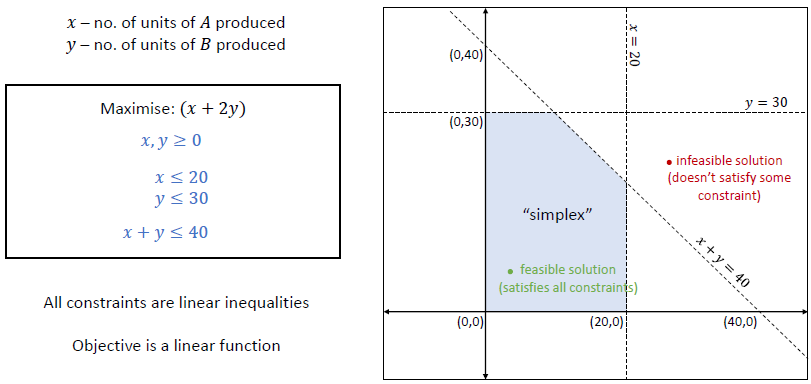
\includegraphics[width=0.7\columnwidth]{simplex}
	\end{center}
	\begin{itemize}
		\item If an optimal solution exist, it will always be at a vertex
		\item There could be situations where linear programs are only constraint in 1 axis $\rightarrow$ feasible solution exists but no optimum, LP is \textbf{unbounded}
		\item Simplex could be roughly described as:
		      \begin{enumerate}
			      \item Start at a feasible vertex, and compute its objective value
			      \item Find a neighbouring vertex with larger objective value
			            \begin{itemize}
				            \item If none exists, output current vertex as  optimum
				            \item Else, move to that vertex and repeat
			            \end{itemize}
		      \end{enumerate}
		\item If optimal solution is\textbf{ parallel with vertex}, any point on the line will be optimal solution
		\item If there are $n$ variables, then simplex will be a $n$-dimensional convex polyhedron
		\item Correctness follows from convexity - any local optimum is a global optimum
	\end{itemize}
	\subsection{Comparison of LP algorithms}
	\begin{center}
		\begin{tabular}{|l|l|}
			\hline
			Algorithms            & Comments                                                                                                                                         \\ \hline
			Simplex Algorithm     & \begin{tabular}[c]{@{}l@{}}Efficient in practice\\ Exponential running time in worst case\end{tabular}                                           \\ \hline
			Ellipsoid Algorithm   & \begin{tabular}[c]{@{}l@{}}First polynomial-time algorithm to solve LP\\ Slow in practice\end{tabular}                                           \\ \hline
			Interior Point method & \begin{tabular}[c]{@{}l@{}}Efficient in practice\\ Polynomial running time in worst case\\ Many recent improvements to running time\end{tabular} \\ \hline
		\end{tabular}
	\end{center}
	\vfill\null\columnbreak
	\section{Reductions}
	Reductions between computational problem is a fundamental idea in algorithm design. It is useful in giving us a way to compare the \textbf{hardness} of 2 problems
	\subsection{Definition of Reduction}
	\begin{itemize}
		\item Consider 2 problems $A$ and $B$. If $A$ can be solved as follows:
		      \begin{itemize}
			      \item \textbf{Input}: Instance $\alpha$ of $A$
			            \begin{enumerate}
				            \item Convert $\alpha$ to an instance $\beta$ of $B$
				            \item Solve $\beta$ and obtain a solution
				            \item Based on solution of $\beta$, obtain solution of $\alpha$
			            \end{enumerate}
			      \item Then, we say $A$ reduces to $B$ $\rightarrow$ Start with $A$, convert to and solve $B$ to obtain solution for $A$
		      \end{itemize}
	\end{itemize}
	\begin{center}
		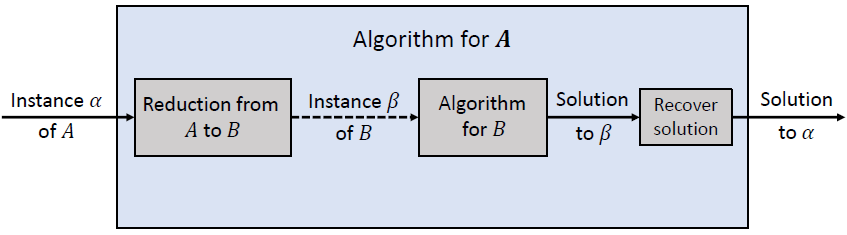
\includegraphics[width=0.7\columnwidth]{reduction}
	\end{center}
	\subsection{Example: Palindrome and LCS}
	\begin{itemize}
		\item Problem
		      $A$: Given string $x$, find its \textbf{Longest Palindromic Subsequence}
		\item Problem
		      $B$: Given pair of strings ($x,y$), find the \textbf{Longest Common Subsequence}
		\item Idea: The LPS of a string is the LCS of the string and its reverse. i.e. LPS $\leq_p$ LCS
	\end{itemize}
	\subsection{Example: T-Sum}
	\begin{itemize}
		\item Problem $A$: Given Array $A$ of length $n$, Output $(i,j)$ such that $A[i]+A[j]=0$
		\item Problem $B$: Given Array $B$ of length $n$, and a number $T$, output $(i,j)$ such that $B[i]+B[j]=T$
		\item Want to show T-Sum $\leq_p$ 0-sum
		\item Idea: Given array $B$, define array $A$ such that $A[i]=B[i]-T/2$. If $(i,j)$ satisfy $A[i]+A[j]=0$ then $B[i]+B[j]=T$
	\end{itemize}
	\subsection{Bounded-Time Reductions}
	Same definition as normal reduction just that the reduction should only take $p(n)$ time and we should be able to obtain the solution of $\alpha$ from $\beta$ in $p(n)$ time as well
	\subsubsection{Encoding of Input}
	\begin{itemize}
		\item In the Palindrome and LCS reduction, it is an $O(n)$ time reduction since a string $x$ will take $O(n)$ bits to represent and reducing it to $(x, rev(x))$ could easily be done in $O(n)$ time where $n$ is the length of string $x$
		\item In Matrix Squaring to Matrix Multiplication reduction, input for squaring is the $N\times N$ matrix and the input for the multiplication is also the same $N\times N$ matrix $\rightarrow O(n)$ reduction where $n=N\times N$
		\item In general $n$ is the \textcolor{red}{length of the encoding of the problem instance}
		\item Integers can be encoded using binary $\rightarrow O(\lg n)$, objects, arrays, matrices are encoded using a list of parameters enclosed in brackets, separated by comma
		\item Note that in the matrices example, the technically correct bits used should be $O(N^2\lg m)$ but we can assume that each element in the matrix is "not too large" i.e. $\leq$ 32 bits so can be treated as constant
	\end{itemize}
	\subsubsection{Running Time Composition}
	\begin{itemize}
		\item Claim that if there is a $p(n)$ time reduction from problem $A$ to problem $B$ and there is a $T(n)$-time algorithm to solve problem $B$ on instances of size $n$, then there is a \[T(p(n))+O(p(n))\] time algorithm to solve problem $A$ on instance of size $n$
	\end{itemize}
	\subsubsection{Polynomial-Time Reduction}
	\begin{itemize}
		\item $A\leq_p B$ if there is a $p(n)$-time reduction from $A$ to $B$ for some \textbf{polynomial function} $p(n)$ $\rightarrow$ implies that $B$ is at least as hard as $A$
		\item If $B$ has a poly time algorithm, then so does $A$
		\item If $A\leq_p B$, we can infer that if $A$ cannot be solved in poly time then neither can $B$
		\item Poly-time algorithms refers to any algorithm that runs in $\leq O(n^5)$
	\end{itemize}
	\subsection{Example: Factor}
	\begin{itemize}
		\item Given 2 positive integers $m$ and $t$, with $t < m$, output whether $m$ is divisible by $f$ such that $1<f\leq t$
		\item \textcolor{red}{Not a poly-time algo!!}
	\end{itemize}
	\begin{center}
		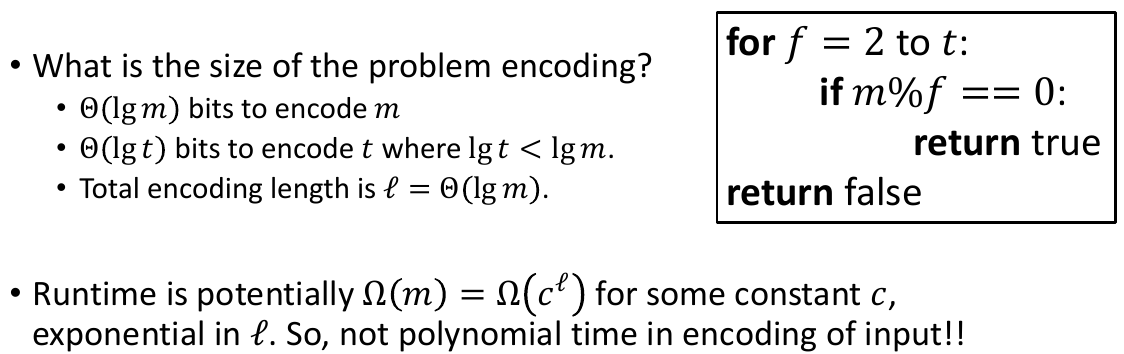
\includegraphics[width=0.7\columnwidth]{factor}
	\end{center}
	\subsection{Knapsack and Fractional Knapsack}
	\begin{center}
		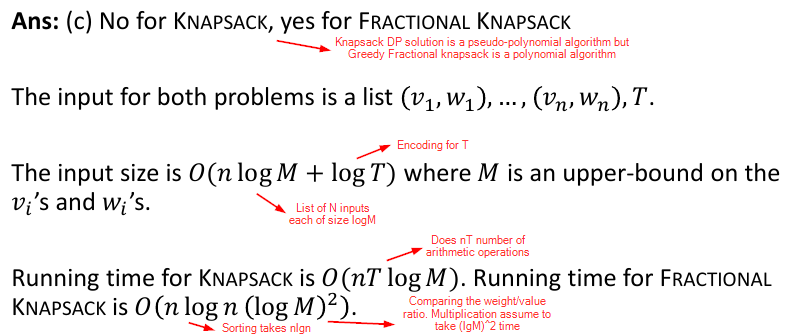
\includegraphics[width=0.8\columnwidth]{knapsack}
	\end{center}
	\subsection{Pseudo-Polynomial Time Algorithm}
	\begin{itemize}
		\item \textbf{Definition}: An algorithm that runs in time polynomial	in the \textbf{\textit{numeric value of the input}} but is exponential in
		      the\textbf{ \textit{length of the representation}} (length in bits) of the input is called a
		      pseudo-polynomial time algorithm
		\item Both factor and knapsack are pseudo-poly time algorithm
		\item \textcolor{red}{Show polynomial in terms of value of input but exponential in terms of length of input!!!}
	\end{itemize}
	\subsection{Decision Problems}
	\begin{itemize}
		\item A decision problem is a function that maps each instance to either "YES" or "NO"
		\item Decision vs Optimization (aka search problems)
		      \begin{itemize}
			      \item \textbf{Decision Problem}: Given a directed graph $G$, is there a path from vertex $u$ to $v$ of length $\leq k$?
			      \item \textbf{Optimization problem}: Given ..., what is the length of the shortest path from $u$ to $v$?
		      \end{itemize}
	\end{itemize}
	\subsubsection{Reducing Decision to Optimization Problem}
	\begin{itemize}
		\item \textbf{decision} $\rightarrow$ \textbf{optimization}:  given an instance of the optimization problem and a number $k$, is there a solution with value $\leq k$?
		\item Decision problem is no harder than the optimization problem $\rightarrow$ given optimal solution, can easily check if $< k$
		\item If we cannot solve optimization problem problem quickly then we cannot solve decision problem quickly $\rightarrow$ decision $\leq_p$ optimization
		\item We \textbf{could also reduce decision problem to Optimization problem} by either sequentially searching for the min/max value which decision problem fails or using binary search
	\end{itemize}
	\subsubsection{Reduction between Decision Problems}
	Given two decision problems $A$ and $B$ , a polynomial-time reduction from $A$ to $B$ denoted $A \leq_p B$  is a transformation
	from instances $\alpha$ of $A$ and $\beta$ of $B$ such that
	\begin{enumerate}
		\item $\alpha$ is a YES-instance of $A$ $\Leftrightarrow$ $\beta$ is a YES-instance from $B$. Could alternatively show YES-instance of $A$ $\rightarrow$ YES-instance of $B$ AND NO-instance of $A$ $\rightarrow$ NO-instance of $B$
		\item The transformation takes polynomial time in the size of $\alpha$
	\end{enumerate}
	\begin{center}
		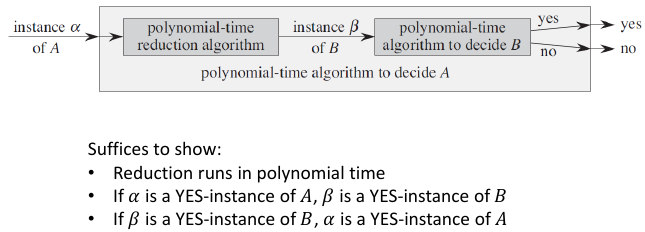
\includegraphics[width=0.7\columnwidth]{a-reduce-b}
	\end{center}
	\section{NP-Completeness}
	\begin{center}
		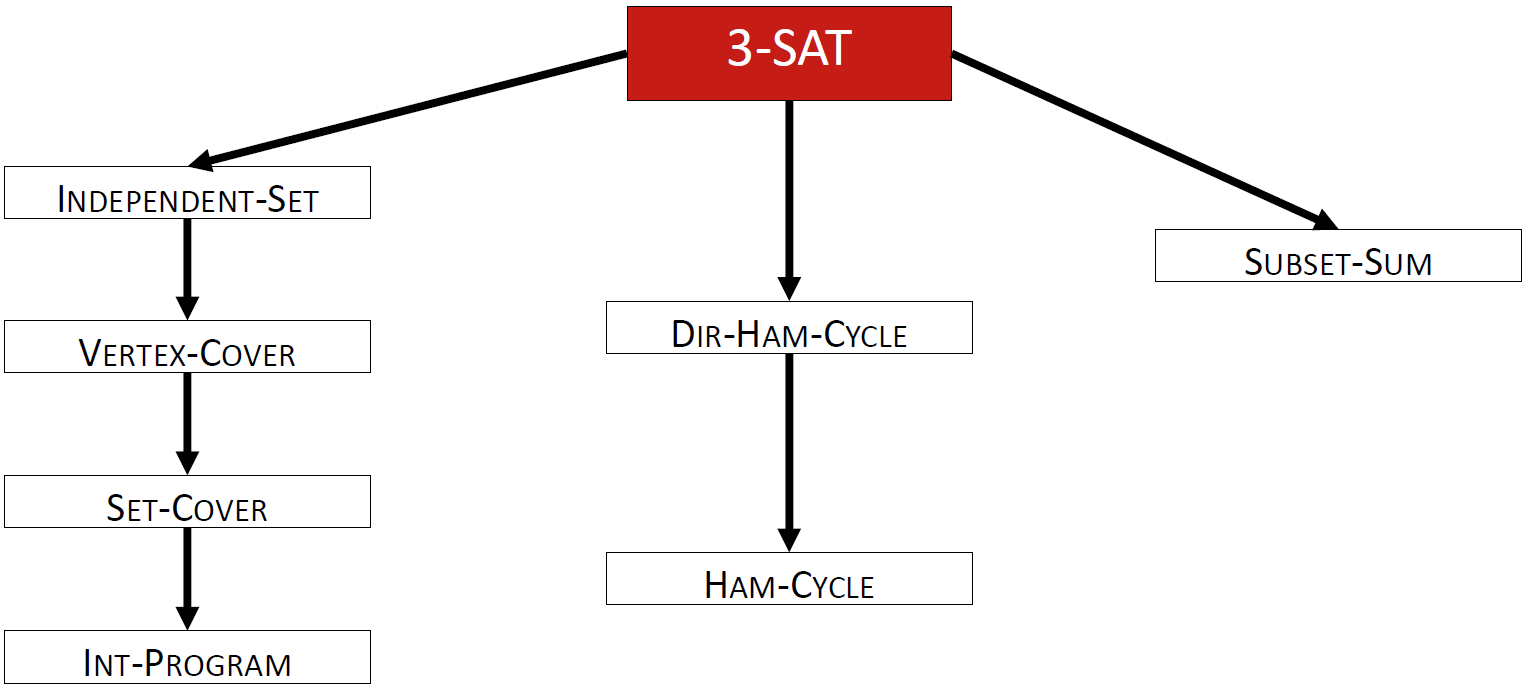
\includegraphics[width=0.7\columnwidth]{reductions}
	\end{center}
	\subsection{Independent Set to Vertex Cover}
	\begin{itemize}
		\item \textbf{Independent-Set}: Given a graph $G=(V,E)$ and an integer $k$, is there a subset of $\geq k$ vertices such that no 2 are adjacent
		\item \textbf{Vertex-Cover}: Given a graph $G=(V,E)$, and an integer $k$, is there a subset of $\leq k$ vertices such that each edge is incident ot at least 1 vertex in the subset
		\item \textbf{Reduction}: Given an instance of $(G, k)$ of independent set, output $(G, n-k)$ as instance of vertex-cover $\rightarrow$ reduction is clearly polynomial since we only change $k$ to $n-k$
		\item  \textbf{YES-instance to YES-instance}
		      \begin{itemize}
			      \item Suppose $G$ has a set of vertices $S$ of size $\geq k$ such that no 2 are connected by an edge
			      \item \textbf{Claim}: $V \backslash S$ is a vertex cover of size at most ($n-k$)
			      \item Let $(u,v)\in E$, then either $u\notin S$ or $v\notin S$. So either $u$ or $v$ will be in $V \backslash S$
		      \end{itemize}
		\item \textbf{NO-instance to NO-instance}
		      \begin{itemize}
			      \item Suppose $(G, n-k)$ is a YES-instance of Vertex-Cover. That is, there is a subset of $S$ of $\leq (n-k)$ vertices that cover all edges
			      \item \textbf{Claim}: $V\backslash S$ is an independent set of size at least $k$
			      \item Let $(u,v)\in E$, if both $(u,v)\in V\backslash S$, then the edge $(u,v)$ is not covered by $S$
			      \item So for any $u\in V\backslash S$, none of its neighbors are in $V\backslash S$, so it is an independent set
		      \end{itemize}
	\end{itemize}
	`	\subsection{Vertex-Cover to Set-Cover}
	\begin{itemize}
		\item \textbf{Set-Cover}: Given integers $k,n$ and a collection $\mathcal{S}$ of subsets of $\{1,...,n\}$, are there $\leq k$ of these subsets who union equals $\{1,...,n\}$
		\item \textbf{Reduction}: Given instance $(G=(V,E), k)$ of Vertex-Cover, we generate an instance $(n,k',\mathcal{S})$ of Set-Cover as follows:
		      \begin{itemize}
			      \item Set $n=|E|$ and $k'=k$
			      \item Order the edges of $G$ arbitrarily: $e_1,...,e_n$
			      \item For each $v\in V$, define subset $S_v=\{i:e_i\text{ incident on }v\}$
			      \item $\mathcal{S}$ is the collection of all such sets $S_v$
		      \end{itemize}
	\end{itemize}
	\begin{center}
		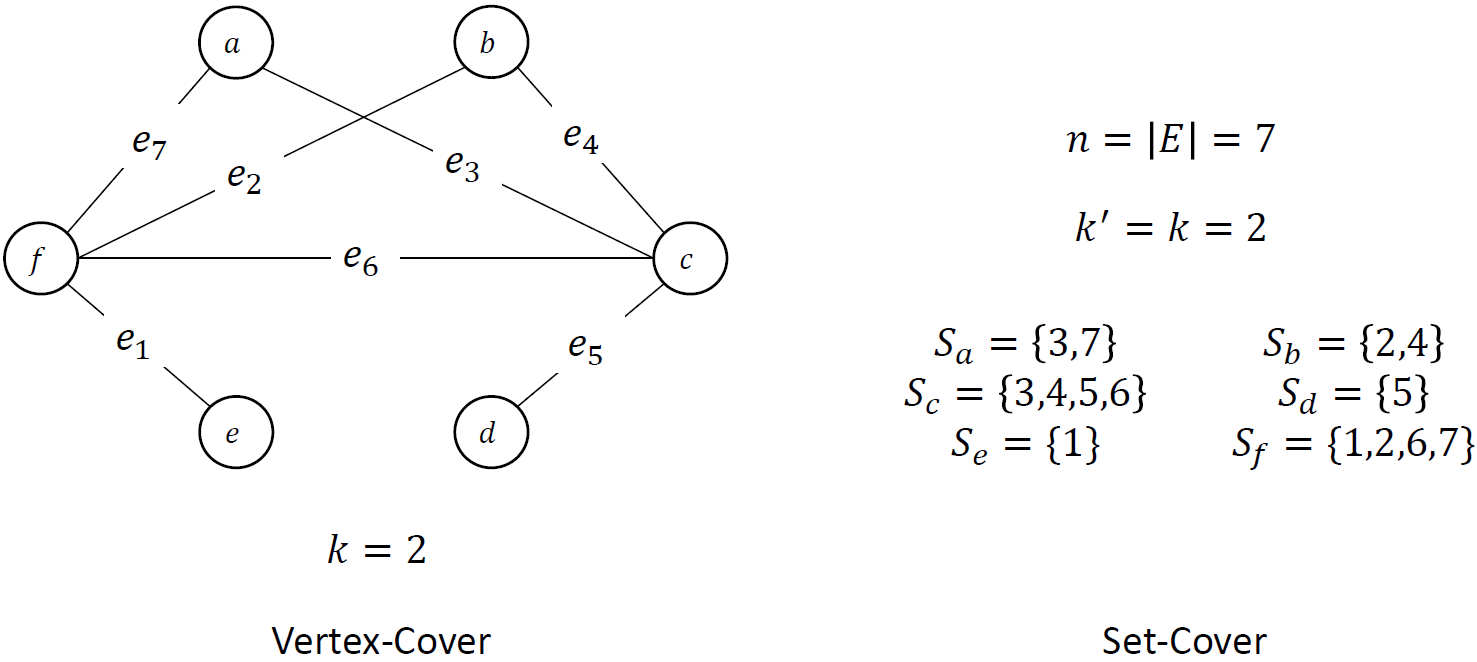
\includegraphics[width=0.6\columnwidth]{vertex-set}
	\end{center}
	\begin{itemize}
		\item \textbf{Running time}:
		      \begin{itemize}
			      \item Polynomial in $|E|$ to order edges
			      \item For each $v\in V$, polynomial time in $|E|$ to write down $S_v$
			      \item Total polynomial time in $|E|$ which is polynomial in the input size
		      \end{itemize}
		\item \textbf{YES-instance to YES-instance}
		      \begin{itemize}
			      \item Suppose $G$ has a vertex-cover $T$ of size $k$, that is every edge in $E$ is adjacent to some $v\in T$
			      \item Each $i$ is contained in $S_v$ if $e_i$ is adjacent to $v$. So the union of $S_v$'s for $v\in T$ contain all $i\in \{1,...,n\}$
			      \item So there is a set of $k$ sets in $\mathcal{S}$ that cover $\{1,...,n\}$, so $(n,k',\mathcal{S})$ is a YES-instance of Set-Cover
		      \end{itemize}
		\item \textbf{NO-instance to NO-instance}
		      \begin{itemize}
			      \item Suppose $(n,k',\mathcal{S})$ is a YES-instance of Set-Cover, that is there is a set $T$ of $k'$ sets from $\mathcal{S}$ that cover $\{1,...,n\}$
			      \item If $i$ is contained in $S_v$ then $e_i$ is adjacent to $v$. So the set of vertices $v$ corresponding to the sets $S_v\in T$ cover all edges $\{e_1,...,e_n\}$
			      \item So $G$ has a vertex cover of size $k$, so $(G,k)$ is a YES-instance of Vertex-Cover
		      \end{itemize}
	\end{itemize}
	\vfill\null\columnbreak
	\subsection{3-SAT to Independent-Set}
	\begin{itemize}
		\item \textbf{SAT}: given a CNF formula $\phi$, does it have a satisfying assignment
		      \begin{itemize}
			      \item Literal: boolean variable and its negation - $x_i, \bar{x_i}$
			      \item Clause: disjunction (OR) of literals - $C_j=x_1 \vee \bar{x_2} \vee x_3$
			      \item Conjunctive Normal Form (CNF): a formula $\phi$ that is a conjunction (AND) of clauses - $\phi=C_1 \wedge C_2 \wedge C_3$
		      \end{itemize}
		\item 3-SAT: SAT where each clause is given in the given formula \textbf{contains exactly 3 literals} corresponding to different variables. Max number of clauses is $2^n$ where $n$ is the number of variables ($x_i$)
		      \begin{itemize}
			      \item Fastest algorithm known for 3-SAT is $1.308^n$ $\rightarrow$ exponential running time
		      \end{itemize}
		\item \textbf{Reduction}:
		      \begin{itemize}
			      \item $G$ contains 3 vertices for each clause - one for each literal
			      \item Connect the 3 literals in each clause in a triangle
			      \item Connect each literal to each of its negation
			      \item Set $k$ = number of clauses
		      \end{itemize}
	\end{itemize}
	\begin{center}
		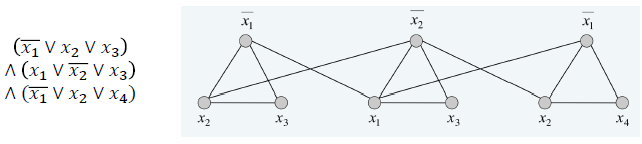
\includegraphics[width=0.6\columnwidth]{3-sat}
	\end{center}
	\begin{itemize}
		\item \textbf{Runtime}: Polynomial in size of $\phi$
		\item \textbf{YES-instance to YES-instance}
		      \begin{itemize}
			      \item If $\phi$ is satisfiable, take any satisfying assignment and, for each clause, some literal that is set to be true by this assignment
			      \item The vertices corresponding to those literals form an independent set of size $k$ $\rightarrow$ the vertices are from different clauses so wont be connected
		      \end{itemize}
		\item \textbf{NO-instance to NO-instance}: \begin{itemize}
			      \item Suppose $(G, k)$ is a YES-instance and has independent set $S$ of size $k$
			      \item Each of the $k$ triangles must contain exactly 1 vertex from $S$
			      \item Set those literals to true and all clauses will be satisfied, so $\phi$ is satisfiable
		      \end{itemize}
	\end{itemize}
	\subsection{Importance of 3-SAT}
	\begin{itemize}
		\item Since \textcolor{red}{reductions are transitive}, if 3-SAT is shown not to have a poly time algorithm, then none of the algorithms will have poly time algorithm
	\end{itemize}
	\subsection{P vs NP}
	\begin{itemize}
		\item \textbf{P}: the class of decision problems solvable in (\textit{deterministic}) polynomial time
		\item \textbf{NP}: !the class of problems for which polynomial-time verifiable certificates of YES-instances
		      exist
		      \begin{itemize}
			      \item aka \textit{non-deterministic polynomial}, no known polynomial time algorithm that solves it but verification can be done in polynomial time
			      \item Verification algorithm is defined as a function $V(x,y)$ that takes an instance $x$ and certificate $y$ with $|y|=poly(|x|)$ such that: there exist a $y$ for which $V(x,y)=1$ iff $x$ is a YES-instance
		      \end{itemize}
	\end{itemize}
	\subsubsection{Problems in P}
	\begin{center}
		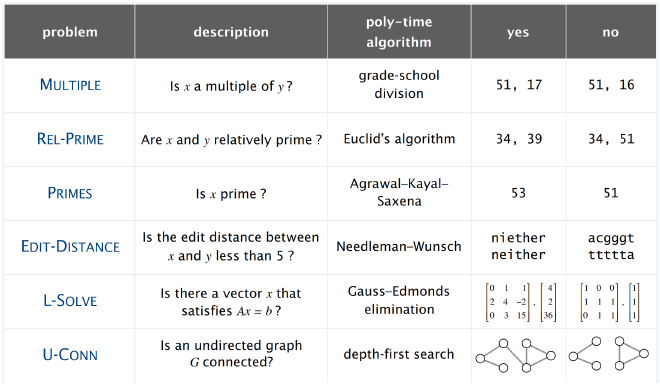
\includegraphics[width=0.7\columnwidth]{p-problems}
	\end{center}
	\subsubsection{Verification Example: Subset-Sum}
	\begin{itemize}
		\item In Subset-Sum, given a list of integers $S$ and target $t$, problem is to decide if there is $S'\subseteq S$ that sums up to $t$
		\item Certificate is the subset $S'$ itself. Verifier checks whether the sum of elements in $S'$ is $t$ in polynomial time
		\item Hence Subset-Sum is in NP.
	\end{itemize}
	\subsubsection{Verification Example: Ham-Cycle}
	\begin{itemize}
		\item In Ham-Cycle, given a graph $G$, problem is to decide whether there is a simple cycle that visits each vertex once
		\item Certificate is the cycle itself. Verifier checks in polynomial time whether it is a cycle and visits each vertex once
		\item Hence, HAM-CYCLE is in NP
	\end{itemize}
	\subsubsection{Verification Example: Factor}
	\begin{itemize}
		\item Given numbers $m$ and $t < m$, is there an $1 < f \leq t$ that divides $m$
		\item Certificate is the number $f$ itself. Verifier checks in poly time if it is $\leq t$
		      and divides $m$
		\item Hence, FACTOR is in NP
	\end{itemize}
	\subsubsection{P $\subseteq$ NP}
	\begin{itemize}
		\item \textcolor{red}{All problem in P is in NP!}
		\item The certificate can be anything. The verifier $V(x,.)$ can solve for the instance $x$ by itself and check if it is a YES-instance
	\end{itemize}
	\subsubsection{co-NP}
	\begin{itemize}
		\item A problem is in co-NP if polynomial time verifiable certificates
		      (“counterexamples”) of NO instances exist
		\item Complement of any NP problem is in co-NP
		\item Factor is also in co-NP, where the certificate for the NO-instance is the prime factorization of $m$. Verifier checks that all factors are more then $t$ and also verifies that they are prime using the AKS primality test
	\end{itemize}
	\subsubsection{NP-Hard \& NP-Complete}
	\begin{itemize}
		\item a problem $A$ is said to be \textbf{NP-Hard} if for every problem $B\in NP$, $B\leq_p A$ $\rightarrow$ $A$ is at least as hard as every problem in NP
		\item a problem $A$ is said to be \textbf{NP-Complete} if it is in \textbf{NP} and is also \textbf{NP-hard}
		\item \textbf{Cook-Levin-Theorem} $\rightarrow$ every problem in NP-Hard can be
		      poly-time reduced to 3-SAT. Hence, 3-SAT is NP-Hard and
		      NP-Complete.
		\item To show a problem is NP-Hard:
		      \begin{enumerate}
			      \item Show that $X$ is in NP $\rightarrow$ YES-instance has a certificate that can be verified in poly time
			      \item Show that $X$ is in NP-Hard $\rightarrow$ show \textcolor{red}{poly-time reduction} from another NP-Hard problem $A$ to $X$
			      \item Show that reduction is valid $\rightarrow$ YES-instance to YES-instance, NO-instance to NO-instance, poly time reduction
		      \end{enumerate}
	\end{itemize}
	\vfill\null\columnbreak
	\section{Approximation Algorithms}
	Previously shown that there are many NP-Complete problems that cannot be solved in poly time but yet they show up often in practice. To deal with them:
	\begin{enumerate}
		\item Use exponential time algorithm (brute force) if a correct answer is required $\rightarrow$ Can be used for small instances
		\item See if given instance has any special features that can make it easier to solve $\rightarrow$ e.g. knapsack with small capacity can be solved using the pseudopoly DP solution
		\item Find an approximation to the problem $\rightarrow$ applicable to \textbf{optimization problems}
	\end{enumerate}
	\subsection{Optimization Problems}
	\begin{itemize}
		\item Vertex-Cover (decision) - asks if there exist a subset of $\leq k$ vertices such that each edge is incident to at least 1 vertex in subset
		\item Vertex-Cover (optimization) - want to find the smallest subset of vertices ...
		\item If optimization can be solved then decision can be solved $\rightarrow$ just check whether optimal solution is less than constraint in decision problem!
		\item If P $\neq$ NP, optimization problem cannot be solved in poly time
	\end{itemize}
	\subsection{Approximating Optimization Problem}
	\begin{itemize}
		\item \textbf{Minimization Problem}: Given an instance, find a solution that has minimum cost
		      \begin{itemize}
			      \item $C^*$: cost of optimal solution
			      \item $C$: cost of solution found by approximation algorithm
			      \item Approximation Ratio: $\frac{C}{C^*}$ $\rightarrow$ always larger than 1. Good approximation algorithm will have small approximation ratio and is ideally a constant
		      \end{itemize}
		\item \textbf{Maximization Problem}:
		      \begin{itemize}
			      \item Approximation ratio will be $\frac{C^*}{C}$ instead
		      \end{itemize}
	\end{itemize}
	\subsection{Approximating Vertex Cover}
	\begin{center}
		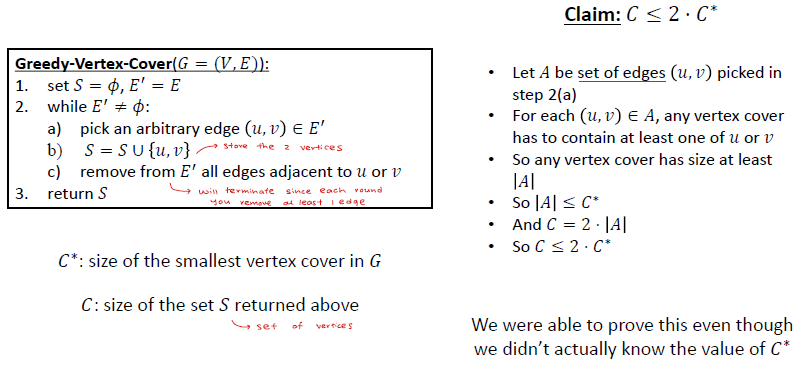
\includegraphics[width=0.7\columnwidth]{vertex-approx}
	\end{center}
	\subsection{Approximating Set Cover}
	\begin{tabular}{l}
		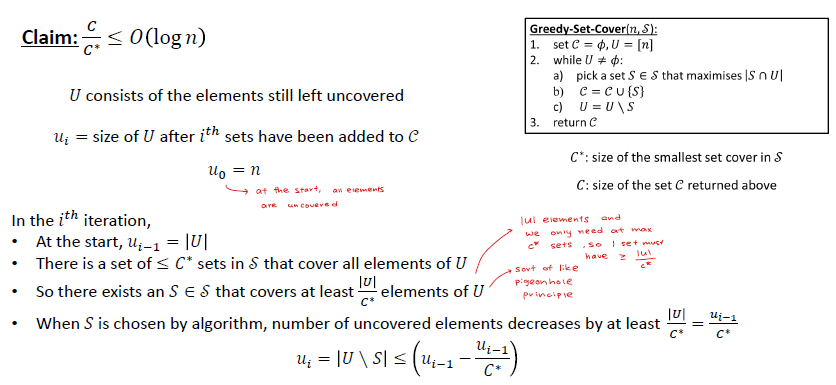
\includegraphics[width=0.48\linewidth]{set-cover-approx1}
	\end{tabular}
	\begin{tabular}{l}
		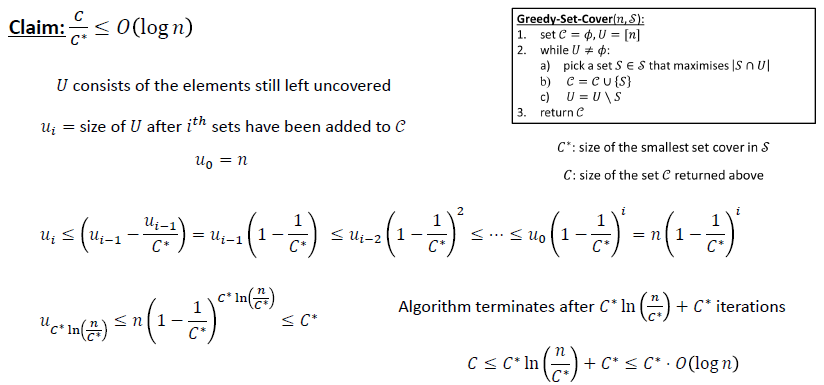
\includegraphics[width=0.48\linewidth]{set-cover-approx2}
	\end{tabular}
	\subsection{Approximating Knapsack}
	Earlier, we used DP to solve Knapsack in pseudo poly time of $O(nW)$. In the approximation algorithm, we use another DP algorithm that solves Knapsack in $O(n^2V)$ where $V$ is the max value of any item
	\begin{itemize}
		\item Need to choose a scaling parameter $k=\epsilon V/n$ for some $\epsilon>0$
		\item $S$ which is the solution given by the approximation algorithm still satisfies the weight constraint since we did not change the weight at all $\rightarrow$ Approximation is $\approx$ optimal!
	\end{itemize}
	\begin{tabular}{l}
		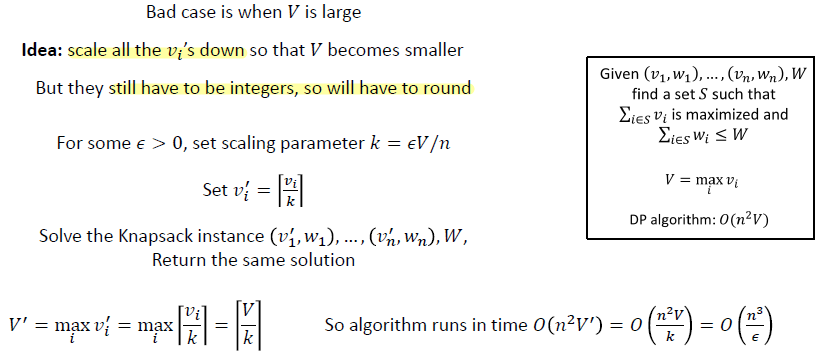
\includegraphics[width=0.48\linewidth]{knapsack-approx}
	\end{tabular}
	\begin{tabular}{l}
		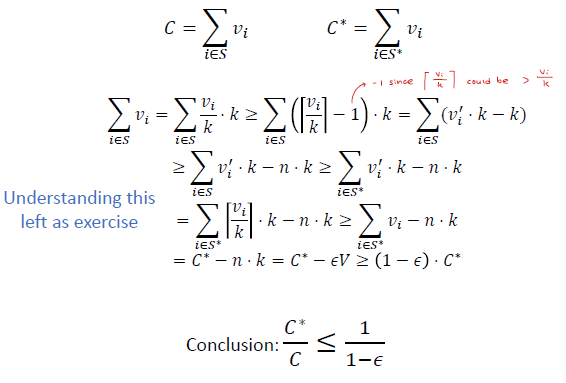
\includegraphics[width=0.48\linewidth]{knapsack-approx-proof}
	\end{tabular}
	\subsection{Approximation Schemes}
	\begin{itemize}
		\item A Polynomial-Time Approximation Scheme (PTAS) for a problem is an algorithm that given an instance and an $\epsilon > 0$, runs in time $poly(n)f(\epsilon)$ for some function $f$ and has approximation ratio $(1+\epsilon)$
		      \begin{itemize}
			      \item Note that $f(\epsilon)$ could be exponential!!
		      \end{itemize}
		\item A Fully Polynomial-Time Approximation Scheme (FPTAS) for a problem is an algorithm that given an instance and an $\epsilon > 0$, runs in time $poly(n, 1/\epsilon)$
		      and has approximation ratio $(1 + \epsilon)$
		\item Approximation algorithm for Knapsack is a FPTAS
	\end{itemize}
	\section{Asymptotic Notations \& Master Theorem}
	\begin{center}
		\textbf{$O$-notation [upper bound ($\leq$)]: $f(n)=O(g(n))$\\}
%		if $\exists c>0,n_0>0$ such that $\forall n\geq n_0$\\
		\fbox{$0\leq f(n)\leq cg(n)$}
		\ \\~\\ \textbf{$\Omega$-notation [lower bound ($\geq$)]: $f(n)=\Omega(g(n))$\\}
%		if $\exists c>0,n_0>0$ such that $\forall n\geq n_0$\\
		\fbox{$0\leq cg(n)\leq f(n)$}
		\ \\~\\ \textbf{$\Theta$-notation [tight bound]: $f(n)=\Theta(g(n))$\\}
%		if $\exists c_1,c_2,n_0>0$ such that $\forall n\geq n_0$\\
		\fbox{$0\leq c_1g(n)\leq f(n)\leq c_2g(n)$}
		\ \\~\\ \textbf{$o$-notation (<): $f(n)=o(g(n))$\\}
%		if $\forall c>0,\exists n_0>0$ such that $\forall n\geq n_0$\\
		\fbox{$0\leq f(n) < cg(n)$}
		\ \\~\\ \textbf{$\omega$-notation (>): $f(n)=\omega(g(n))$\\}
%		if $\forall c>0,\exists n_0>0$ such that $\forall n\geq n_0$\\
		\fbox{$0\leq cg(n) < f(n)$}
	\end{center}
	\ \\ \textcolor{red}{Note: $\Theta(g(n))=O(g(n))\cap{\Omega(g(n))}$}
	\subsection{Limits}
	\begin{minipage}{0.45\columnwidth}
		\begin{center}
			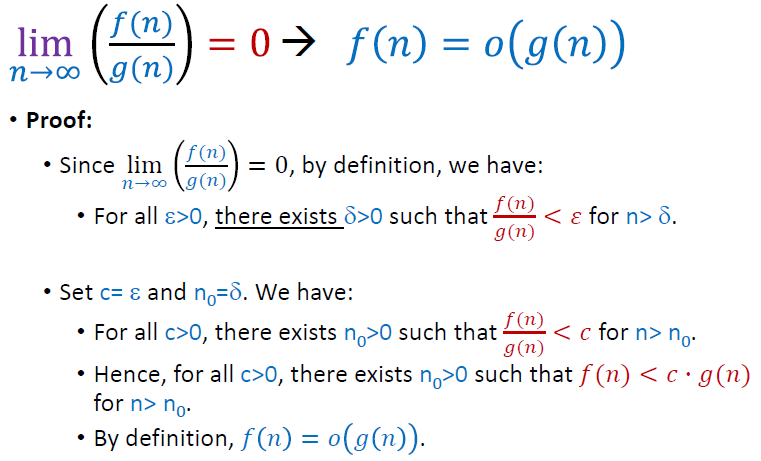
\includegraphics[width=1\columnwidth]{proof_delta_epsilon}
		\end{center}
	\end{minipage}
	\begin{minipage}{0.55\columnwidth}
		Assume $f(n),g(n)>0$
		\begin{align*}
			&\lim\limits_{n \to \infty} \frac{f(n)}{g(n)} = 0 &\Rightarrow f(n) = o(g(n)) \\
			&\lim\limits_{n \to \infty} \frac{f(n)}{g(n)} < \infty &\Rightarrow f(n) = O(g(n)) \\
			0 < &\lim\limits_{n \to \infty} \frac{f(n)}{g(n)} < \infty &\Rightarrow f(n) = \Theta(g(n)) \\
			&\lim\limits_{n \to \infty} \frac{f(n)}{g(n)} > 0 &\Rightarrow f(n) = \Omega(g(n)) \\
			&\lim\limits_{n \to \infty} \frac{f(n)}{g(n)} = \infty &\Rightarrow f(n) = \omega(g(n))
		\end{align*}
	\end{minipage}
	\subsection{Common useful facts}
	\begin{itemize}
%		\item if $f(n) = \omega(g(n))$, then $f(n) = \Omega(g(n))$
%		\item if $f(n) = o(g(n))$, then $f(n) = O(g(n))$
%		\item Degree-\textit{k} polynomials are $O(n^k)$.
%		\item Degree-\textit{k} polynomials are $o(n^{k+1})$ and $\omega{(n^{k-1})}$.
%		\item \textcolor{red}{Poly dominates logs:} $(\log{n})^{100}=o(n^{.0001})$, i.e. $n^k > (\log{n})^k$
%		\item \textcolor{red}{Exponential dominate polys:} $n^{100}=o(2^{.001n})$, i.e. $2^{kn}>n^k$
		\item \hl{$1 < \log\log n < \log n < (\log n)^k < \sqrt{n} < n < n^k < a^n < n! < n^n$}
		\item $2^{2\cdot2^{\lg\lg n}}<n^2\lg\lg n<n^3\equiv\sum_{i=2}^{n}\dfrac{n^3}{i(i-1)}<n^{\lg n}<2^n<(\lg n)^n<n!$
	\end{itemize}
	\subsection{Master Method}
	\begin{math}
		T(n) = aT(\frac{n}{b}) + f(n) = \begin{cases}
			\Theta(n^{\log_ba}) & \text{ if } f(n) < n^{\log_ba} \text{ polynomially}
			\\ \Theta(n^{\log_ba} \log n) & \text{ if } f(n) = n^{\log_ba} 
			\\ \Theta(f(n)) & \text{ if } f(n) > n^{\log_ba} \text{ polynomially}
		\end{cases}
	\end{math} 
	where $a\geq 1, b>1$ and $f$ is asymptotically positive
	\textbf{3 common cases of Master Method}
	\begin{enumerate}
		\item If $f(n) = O(n^{\log_b a-\varepsilon})$ for some constant  $\varepsilon > 0$, 
		\begin{itemize}
			\item $f(n)$ grows polynomially slower than $n^{\log_ba}$ by $n^\varepsilon$ factor.
			\item then $T(n) = \Theta(n^{\log_ba})$.
		\end{itemize}
		\item If $f(n) = \Theta(n^{\log_ba} \log^kn) $ for some $k \geq 0$,
		\begin{itemize}
			\item $f(n)$ and $n^{\log_ba}$ grow at similar rates.
			\item then $T(n) = \Theta(n^{\log_ba}\log^{k+1} n)$
		\end{itemize}
		\item If $f(n) = \Omega(n^{\log_ba + \varepsilon})$ for some constant $\varepsilon > 0$, 
		\begin{itemize}
			\item and $f(n)$ satisfies the \textbf{regularity condition} 
			\begin{itemize}
				\item $af(n/b) \leq cf(n)$ for some constant $c<1$ and all sufficiently large $n$
				\item this guarantees that the sum of subproblems is smaller than $f(n)$.
			\end{itemize} 
			\item $f(n)$ grows polynomially faster than $n^{\log_ba}$ by $n^\varepsilon$ factor
			\item then $T(n) = \Theta(f(n))$.
		\end{itemize}
	\end{enumerate}
	\section{Miscellaneous}
	\subsection{Useful Facts}
	\begin{multicols*}{2}
		\begin{itemize}
			\item $e^x\geq 1+x$
			\item $ (1-\dfrac{1}{n})^n\approx\dfrac{1}{e} $
			\item $\sum\limits_{j=0}^{\lg(n-1)}2^j=2^{\lg(n-1)+1}-1\\ \hspace*{4em}\leq{2(n-1)}$
			\item $a=b^{\log_ba}$
			\item $\log_c(ab)=\log_ca+\log_cb$
			\item $\sum\limits^{\lg n}_{i=0}\dfrac{1}{\lg n/{a^i}} = \lg\lg n$
			\item $(\lg n)!\leq \lg n^{\lg n}=2^{\lg n \lg\lg n}$
			\item $\sum_{i=1}^{\lg n}\lg\lg \frac{n}{i}=\lg n\lg\lg n$
			\item $\log_ba^n=n\log_ba$
			\item $\log_ba=\dfrac{\log_ca}{\log_cb}$
			\item $\log_b(1/a)=-\log_ba$
			\item $\log_ba=\dfrac{1}{\log_ab}$
			\item $a^{\log_bc}=c^{\log_ba}$
			\item $\dfrac{d}{dn}\lg\lg n = \dfrac{1}{n\lg n}$
			\item $n^2\log_nn!=n^2\times \frac{\lg n!}{\lg n}=n^3$
		\end{itemize}
	\end{multicols*}
	\subsection{Approximations and Series}
	\begin{itemize}
		\item Stirling's Approximation:
		\begin{itemize}
			\item $n!=\sqrt{2\pi n}(\dfrac{n}{e})^n(1+\Theta(\dfrac{1}{n}))$
			\item $\log(n!)=\Theta(n\log n)$
		\end{itemize}
		\item Arithmetic Series: $\sum_{k=1}^n=1+2+3+\cdots+n=\dfrac{1}{2}n(n+1)=\Theta(n^2)$
		\item Harmonic Series: $\sum^n_{k=1}\dfrac{1}{k}=\Theta(\lg(n))$
		\item Geometric Series: $\sum_{k=0}^nx^k=1+x+x^2+\cdots+x^n=\dfrac{x^{n+1}-1}{x-1}$
		\item Geometric Series: $\sum_{k=0}^\infty x^k=\dfrac{1}{1-x}$ when $|x| < 1$
		\item L'Hopital's Rule: $\lim\limits_{x \to \infty}\dfrac{f(x)}{g(x)}=\lim\limits_{x \to \infty}\dfrac{f'(x)}{g'(x)}$
	\end{itemize}
	\subsubsection{Arithmetic and Geometric Series}
	\begin{center}
		\begin{tabular}{|c|c|c|}
			\hline
			& Arithmetic                  & Geometric                                \\\hline
			$a_n$           & $a_n=a_1+d(n-1)$            & $a_n=a_1\cdot r^{n-1}$                   \\\hline
			$S_n$           & $S_n=\dfrac{n}{2}(a_1+a_n)$ & $S_n=a_1\left(\dfrac{1-r^n}{1-r}\right)$ \\\hline
			Infinite Series &                             & $S_\infty=\dfrac{a_1}{1-r}$, |$r$| < 1   \\\hline
		\end{tabular}
	\end{center}
	\subsection{Permutations and Combinations}
	\begin{itemize}
		\item nPr = n! / (n-r)!
		\item nCr = n! / (n-r)!r!
		\item $\binom{2n}{n}\approx2^{2n}/\sqrt{n}$
	\end{itemize}
\end{multicols*}
\end{document}
